\documentclass[12pt]{article}
\usepackage{float}
\usepackage[margin=2cm]{geometry}
\usepackage{graphicx}
\usepackage{hyperref}
\hypersetup{colorlinks=true, urlcolor=blue}

\title{\huge{Sensitivity of shoreline-trajectory to deposition-events}
\Large{Accuracy of inferred signal as function of signal-shape and sample-rate\\}
\large{Implications for Sequence-Stratigraphy}}
\author{Daniel Mikes}
\date{October 2024}

\begin{document}

\maketitle

\section*{Summary}

Sequo-Strat (Sequence Stratigraphy) is a method that has many applications, the essence of which seems to be: (1) correlate depo-units (deposition units) to depo-units and (2) correlate depo-units to sea-level. These build respectively on following premises: (1) depo-units are laterally continuous and (2) depo-units are sufficiently frequent. For the sake of simplicity, this work focuses solely on the sensitivity of sample-rate on reliability of inferred sea-level from depo-events. It shall consist of three parts: (1) Sea-level signal mimics insolation-curve over $1Ma$; (2) Samples are taken randomly in a wide range ($1-1000$); (3) Ratio of inferred cycles / original cycles is used as measure of fit. This is done for default set of parameter values for insolation, i.e. Period $T$, Amplitude $A$, Period-Modulator $T_m$, Amplitude-Modulator $A_m$, Phase $p$ for Eccentricity $s_E$, Obliquity $s_\theta$, Precession $s_\omega$: insolation $s$ ($T_E=100ka$, $T_\theta=41ka$, $T_\omega=26ka$, $A_E=2$, $A_\theta=25$, $A_\omega=15$, $T_m=5T$, $A_m=\frac{1}{2}A$, $p=0$). The curve of fit (linear scale) against sample-rate (logarithmic scale) matches a logistic curve. The simulation is then performed for all combinations of parameter values within their range. These results provide a spread around the logistic-curve for default values. Samples represent clusters of depo-events. The results do not simulate real processes, they treat the essence of the matter in a conceptual manner. The question is now: if one were to transfer these findings to natural depo-systems, how would they affect the use of Sequo-Strat?

\section*{Key-Words}

delta, depo-event, deposition-event, eustatic sea-level, sample, sequence-stratigraphy, sequo-strat, shoreline-trajectory, signal, tectonic subsidence

\section*{Introduction}

In order to infer signal from samples in general or sea-level from shoreline-trajectory in special one must: (1) Know the shape of the signal and (2) Take sufficient samples from it. This seems quite an ambitious goal for the case of sea-level and depo-events. And it seems to be the exact opposite of what one does in Sequo-Strat, since one infers sea-level from shoreline-trajectory, implicitly assuming that all conditions have been met to reliably do so. Should it not be a requirement to use the method only if all those conditions have explicitly been verified? It is outside the scope of this work to evaluate them all, but for the sake of introduction to the context one shall briefly discuss them. The questions that should always be asked are: (1) Is sea-level curve known? (2) Are depo-events sufficiently frequent?

Relative sea-level can be considered the result of an interplay of three main factors: (1) Tectonic Subsidence, (2) Eustatic Sea-Level, (3) Supply-Rate at the delta-apex. In order to know relative sea-level one must know all three composing factors. Is it safe to assume any of those to be constant and therefore relative sea-level to be governed by only one? Consider a deltaic depo-system, that deposits at the shoreline and therefore records shoreline position. Connect those shorelines and obtain shoreline-trajectory. Is it safe to assume depo-events to be sufficiently frequent and shoreline-trajectory to follow relative sea-level so its shape to be direct reflection of sea-level?

\subsection*{Tectonic Subsidence $Y$}

Tectonic Subsidence can be considered the result of interplay of four main mechanisms. Their manifestation varies substantially in magnitude and time-scale. Isostatic rebound is notable, because it occurs as result of heating or cooling, but also as result of loading or unloading, both of which occur even on passive margins, particularly where deltaic depo-systems deposit significant amounts of sediment.

$$
Y(t) = f(R,M,\sigma,q)
$$

\begin{itemize}
  \item isostasic rebound $R$
  \item bending moment $M$
  \item intraplate stress $\sigma$
  \item heatflux $q$
\end{itemize}

\subsection*{Insolation $I$}

Insolation can be considered the result of interplay of three sine waves, all three related to changes in orbital behaviour of earth around sun. Because their amplitudes vary and because they are not harmonics, the result is an irregular signal, very much different from a single sine wave as is often depicted on Sequo-Strat schematics. To infer such irregular signal from samples requires much more samples than for a single sine wave.

$$
I(t) = f(E,\theta,\omega)
$$

\begin{itemize}
  \item eccentricity $E$
  \item obliquity $\theta$
  \item precession $\omega$
\end{itemize}

\subsection*{Absolute Sea-level $L$}

Absolute Sea-Level fluctuation can be considered to be caused by insolation fluctuations: insolation affects global temperature, which in turn affects global sea-level. But between cause and effect is a long chain of mechanisms. Therefore absolute sea-level can be considered the result of an interplay of all these mechanisms. Is it safe to assume absolute sea-level to mimic the insolation curve? Given the number of mechanisms in that chain, is it safe to assume they would cause no such effects as attenuation, filtering or smoothing?

$$
L(t) = f(T,\Omega,Q,P,E)
$$

\begin{itemize}
  \item temperature $T$
  \item polar ice $\Omega$
  \item polar transport $Q$
  \item continent precipitation $P$
  \item ocean evaporation $E$
\end{itemize}

\subsection*{Relative Sea-Level $\tilde{L}$}

Relative Sea-Level can be considered the result of an interplay of two factors.

$$
\tilde{L}(t) = f(Y,L_E)
$$

\subsection*{Deposition $D$}

Deposition can be considered on two spatially distinct scales: (1) Regional Supply-Rate; (2) Local Supply-Rate. First can be considered the result of an interplay of external (allogenic) factors. Second can be considered the result of an interplay of external (allogenic) and internal (autogenic) factors.

\subsubsection*{Regional Supply-Rate}

Regional Supply-Rate fluctuations can be considered to be caused by insolation fluctuations: insolation affects global temperature, which in turn affects regional supply-rate. But between cause and effect is a long chain of mechanisms. Therefore regional supply-rate can be considered the result of an interplay of all these mechanisms. Is it safe to assume regional supply-rate to be continuous or at least clusters of depo-events to be sufficiently frequent to adequately sample sea-level curve? Is it safe to assume they would cause no non-linear behaviour of any kind? Is it safe to assume supply-rate to delta-apex to be continuous or at least linearly correlated to global temperature?

$$
D(t) = f(T,P,W,R,Q)
$$

\begin{itemize}
  \item temperature $T$
  \item precipitation $P$
  \item weathering $W$
  \item erosion $R$
  \item transport $Q$
\end{itemize}

\subsubsection*{Local Supply-Rate}

Local Supply-Rate fluctuations can be considered to be caused by a host of factors and mechanisms, all of which are very specific to the area and subject to temporal and spatial variation. Deposition and Erosion happen by way of instantaneous events seen on geological time-scale. It is therefore obvious that deposition is not continuous, neither spatially nor temporally. The question is rather how depo-events are spread over space and time. Is it safe to assume them to be equally and densely distributed over time? Or are they more likely to occur in clusters? And should we consider those clusters as samples?

$$
D(t) = f(S,E,D)
$$

\begin{itemize}
  \item Lobe-Switching $S$
  \item Erosion $E$
  \item Deposition $D$
\end{itemize}

\subsection*{Shoreline-trajectory $X$}

Shoreline-Trajectory can be considered to mimic Relative Sea-Level-Curve, but only if depo-events (or clusters of depo-events) are sufficiently frequent. But even if they would be, is it safe to assume them to be mirror-images? Even under steady sea-level and constant deposition, shoreline moves out horizontally. One can depict this graphically by using lateral position from delta-apex together with angle-of-climb of subsequent shoreline positions. Maybe one should rather focus on number of cycles in both signals rather than on exact shape.

$$
X(t) = f(L,D)
$$

\section*{Simulation}

This work shall only focus on the most elementary yet essential of all factors on signal inference, that of sample-rate. The input shall be composite sine wave of three sine waves. The variable shall be sample-rate. The metric shall be number of cycles in original and inferred signal. The immediate goal is to determine sensitivity of signal-inference to sample-rate. Rationale behind this choice is that whatever the shape of the sea-level curve, be it similar to or different from insolation-curve, sample-rate is essential to infer the signal adequately.

\subsection*{Premises}

Premises for this work are in the form of simplifications: (1) Tectonic Subsidence is steady, (2) Absolute Sea-Level mimics Global Temparature, (3) Global Temperature mimics Insolation.

$$
Y'(t) = 0
$$

$$
L(t) = T(t)
$$

$$
T(t) = I(t)
$$

Under those simplifications the following conditions occur: (1) Global Sea-Level mimics Insolation, (2) Relative Sea-Level mimics Global Sea-Level, (3) Relative Sea-Level mimics Insolation.

$$
L(t) = I(t)
$$

$$
\tilde{L}(t) = L(t)
$$

$$
\tilde{L}(t) = I(t)
$$

\subsection*{Signal}

The input-signal is that of Insolation (\autoref{fig:insolation}), which is a composite sine-wave of three sine-waves: (1) Eccentricity, (2) Obliquity, (3) Precession. Duration of signal for all simulations is $1Ma$.

$$
L(t) = A_E sin(f_E t + \phi_E) + A_\theta sin(f_\theta t + \phi_\theta) + A_\omega sin(f_\omega t + \phi_\omega)
$$

\begin{itemize}
  \item Period $T$
  \item Amplitude $A$
  \item Period modulator $T_m$
  \item Amplitude modulator $A_m$
  \item phase $p$
\end{itemize}

\subsubsection*{Constant Parameters}

Default values for parameters are given in following table. Period is in years, amplitude has no dimension, phase is in radians. These are used for the default-scenario, where sample-rate is the only independent variable (\autoref{fig:constant}).

\begin{table}
\centering
\caption{Default paramater values}
\label{tab:default}
\begin{tabular}{c|c|c|c|c}
& $E$ & $\theta$ & $\omega$ & \\
\hline
$T$ & $1.0 \cdot 10^5$ & $4.1 \cdot 10^4$ & $2.6 \cdot 10^4$ & $a$ \\
$A$ & $0.2$ & $2.5$ & $1.5$ & - \\
$T_m$ & $5 \cdot T_E$ & $5 \cdot T_\theta$ & $5 \cdot T_\omega$ & $a$ \\
$A_m$ & $0.5$ & $0.5$ & $0.5$ & - \\
$p$ & 0 & 0 & 0 & rad \\
\end{tabular}
\end{table}

\subsubsection*{Variable Parameters}

Ranges of parameter values are given in following table. These are used for all other scenarios, where parameter values are varied within their range (\autoref{fig:variable}).

\begin{table}
\centering
\caption{Parameter ranges}
\label{tab:range}
\begin{tabular}{c|c|c|c|c}
& $min$ & $max$ & $step$ & \\
\hline
$T$ & $2^2$ & $2^4$ & $1$ & $10^4a$ \\
$A$ & $0$ & $25$ & $5$ & - \\
$T_m$ & $2^0$ & $2^2$ & $1$ & $10^5a$ \\
$A_m$ & $0$ & $12$ & $2.5$ & - \\
$p$ & $2^{-3}$ & $2^{-1}$ & 1 & $\pi$ \\
\end{tabular}
\end{table}

\subsection*{Sample}

Sample-rate is given as number of samples over duration of signal. A complete run for default scenario consists of following steps: (1) run simulation for constant set of parameter values and constant sample-rate; (2) repeat 10 times; (3) increase sample rate. For the runs with variable parameter these are performed for all permutations of parameter values. Samples are taken at random moments over time. These samples are then evenly distributed over time. This has no effect on number of cycles, but is meant to represent real practice between two known time-lines. Original samples and shifted samples are plotted (\autoref{fig:simulation}).

$$
D(t) = f(U)
$$

$$
U \in \{1 \cdot 10^1,1 \cdot 10^3\}/10^5a
$$

- Sample-Rate $U$

\subsection*{Sensitivity}

Plots depict fit against sample-rate. Fit is ratio of number of cycles in sample-signal over number of cycles in original signal.

$$
F = \frac{N_D}{N_L}
$$

\section*{Conclusion}

\subsection*{Analysis}

Fit against sample-rate on a log-linear scale matches a logistic function (\autoref{fig:constant}). Therefore sample-rate directly determines how many cycles of original signal are captured by sampling. Variations in signal-parameters only cause a spread around the default-scenario (\autoref{fig:variable}). These curves give clear numbers on how many samples are required for specific fit. Fit for 60 samples is only $\frac{1}{2}$, fit for 120 samples is $\frac{3}{4}$.

\subsection*{Synthesis}

This work addresses the essential element of the signal-inference problem: how many samples are required to capture the signal adequately? For the case of a known single sine-wave with known regular sampling the answer is quite different from that of an unknown signal with unknown irregular sampling. For use of Sequo-Strat it seems that the former is implicitly adopted, whereas the latter should explicitly be adopted. Relative Sea-Level is unknown and is unlikely to mimic Insolation. Tectonic Subsidence is unlikely to be constant. Depo-Events are unlikely to be regular and sufficiently frequent to capture sea-level fluctuations. These factors require careful scrutiny and any study performing correlation of any kind, be it in space-domain or time-domain, should explicitly address all simplifications or assumptions taken and attempt to assess their implications.

\subsection*{Code}

The code for this work is written in Jupyter/Python and is available on GitHub (\url{https://github.com/danmikes/samsim}). Feel free to use and modify it. Maybe this could lead to a collective effort to quantify relevant parameters and assess accuracy of spatial and temporal correlation in depo-systems.

\subsection*{Figure}

\begin{figure}[hbtp]
\centering
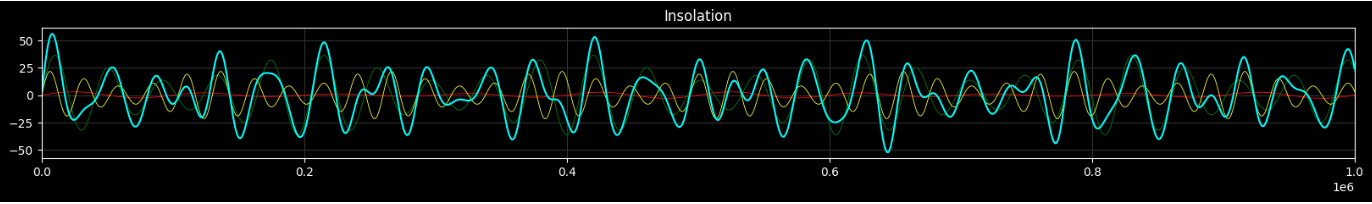
\includegraphics[width=\textwidth]{insolation.png}
\caption{Insolation curve for default parameter values. Red = Eccentricity. Green = Obliquity. Yellow = Precession. Cyan = Insolation.}
\label{fig:insolation}
\end{figure}

\begin{figure}[hbtp]
\centering
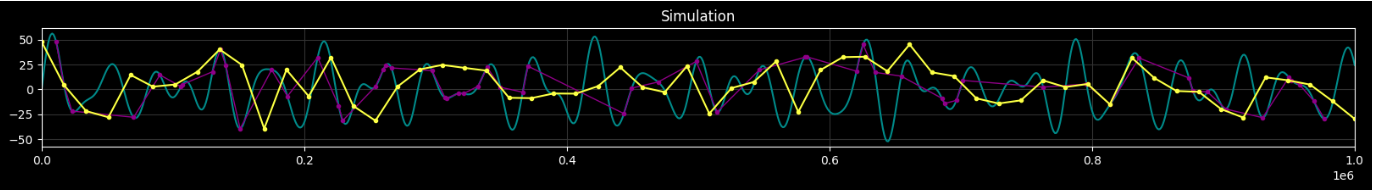
\includegraphics[width=\textwidth]{simulation.png}
\caption{Simulation for default parameter values and sample-rate = 65. Cyan = Insolation. Magenta = Samples. Yellow = Evenly distributed samples.}
\label{fig:simulation}
\end{figure}

\begin{figure}[hbtp]
\centering
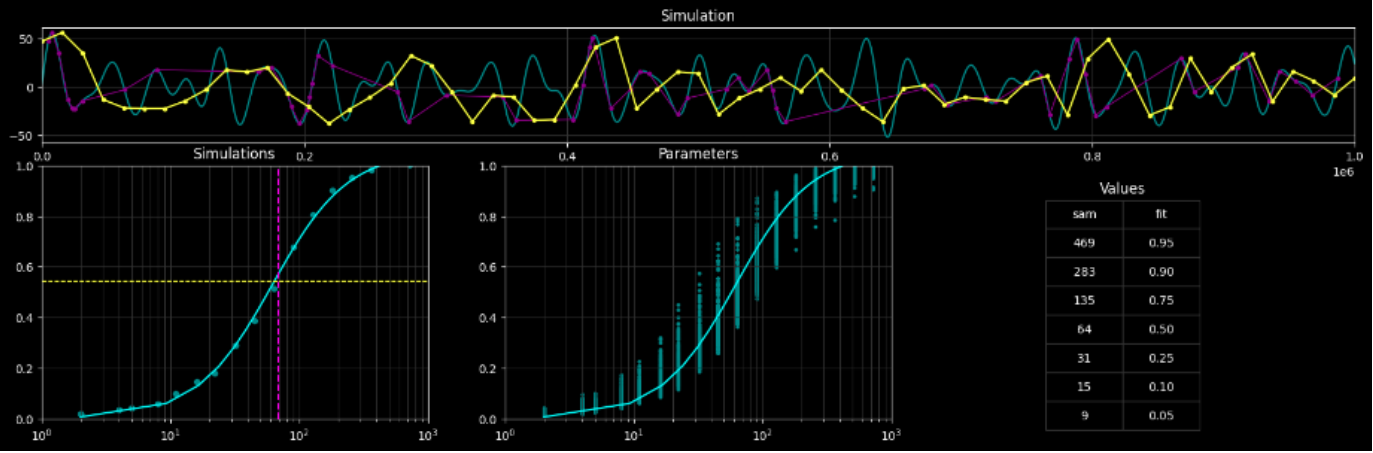
\includegraphics[width=\textwidth]{constant.png}
\caption{Simulation = Simulation for default parameter values and sample-rate = 65. Simulations = Simulation for range of sample-rates and logistic-function matching results. Parameters = Simulation for range of sample-rates and range of Amplitude-values with matching logistic-curve. Lower-Right gives values. Logistic = max, dip, flex for logistic-fit of simulations with default parameter values. Simulation shows minimum, average, maximum sample-rate and fit for simulation with default parameter values. Variable shows minimum, average, maximum sample-rate and fit for simulation with varying amplitude.}
\label{fig:constant}
\end{figure}

\begin{figure}[hbtp]
\centering
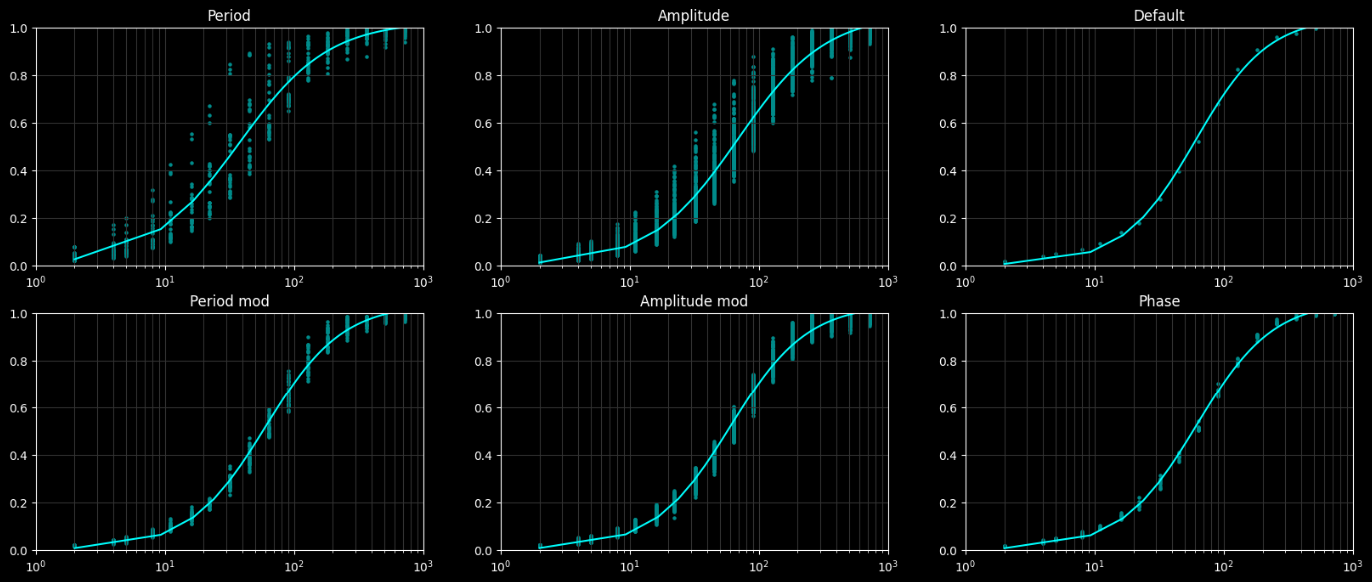
\includegraphics[width=\textwidth]{variable.png}
\caption{Results for variable parameters (\autoref{tab:range}) with matching logistic-function results. For the ranges chosen Period and Amplitude have most effect, Period modulator and Amplitude modulator have intermediate effect and phase has least effect. Default plot shows results for simulation with default parameter values.}
\label{fig:variable}
\end{figure}

\end{document}
